Two test examples presented for 1-D compressible gas flow in a porous media. Analytical solution exists for both under the steady state condition. The first test case is dealing with density changing with pressure only, i.e. isothermal case (sec. \ref{bmt:Isothermal_compressible_flow}). The second example shows Joule-Thomson processes with heat dissipation during carbon sequestration and enhance gas recovery.
\subsection{Isothermal compressible gas flow}
\label{bmt:Isothermal_compressible_flow}
\subsection{Definition}
We consider a simple 1D test example where gas is injected at constant pressure into the porous medium. The material
parameters are summarized in Tab. \ref{tab:compressible_test}.
\subsection{Solution}
\subsubsection{Analytical solution}
For isothermal flow with Dirichlet boundary conditions, i.e. $p(x=0, t)=p_1$ and $p(x=L, t)=p_2$, there exists an analytical solution,
\begin{equation}
p(x)=\sqrt{(p_2^2-p_1^2)\frac{x}{x_2-x_1}+p_1^2}
\label{eqn:press_analytical}
\end{equation}
which is used for verification of the present numerical solution.


According to Darcy's law (\ref{eqn:darcy_gas}) the volumetric gas flux at reference conditions can be approximated as follows
\begin{equation}
Q_0
=
A
\frac{T_0}{T^* p_0}
\frac{\k}{\mu}
\frac{(p_2^2-p_1^2)}{2(x_2-x_1)}
\label{eqn:gasflux_analytical}
\end{equation}
\begin{table}[htb]
\caption{\label{tab:compressible_test}Model parameters.}
\begin{center}
\begin{tabular}{llrr}
\toprule
Symbol & Parameter & Value & Unit \\
\midrule
$L$ & Model length & $100$ & $\mathrm{m}$\\
$A$ & Cross section area & $1$  & $\mathrm{m^2}$ \\
$n$ & Porosity & $0.35$  & $-$ \\
$\k$ & Permeability & $2.7\times 10^{-11}$ & $\mathrm{m^2}$\\
$\mu$ & Gas dynamic viscosity & $1.76\times 10^{-5}$ & $\mathrm{Pa~s}$\\
$p_0$ & Initial condition & $101325$ & $\mathrm{Pa}$\\
$p_1, p_2$ & Boundary conditions & $3 \times 10^6, 1.01325 \times 10^5$ & $\mathrm{Pa}$\\
$\Delta t$ & Time step & $1,10,10^2,10^3,10^4$ & $\mathrm{s}$\\
$\Delta x$ & Space step & $1$ & $\mathrm{m}$\\
\bottomrule
\end{tabular}
\end{center}
\end{table}
\subsubsection{Numerical solution}
The numerical model consists of $100$ line elements connected by $101$ nodes along the x-axis. The distances of the nodes $\Delta x$ is one meter. At $x=0~\mathrm {m}$ there is a constant pressure boundary value is $3 \times 10^6~\mathrm {Pa}$. Whereas at $x=L$ pressure boundary value is $1.01325 \times 10^5~\mathrm {Pa}$.
\begin{figure}
\centering
\includegraphics[scale=0.3]{PART_II/G/gas_flow_new.eps}
\caption{\label{fig:air_steady}Comparison of analytical ($\bullet$) and numerical solutions.}
\end{figure}
\subsection{Results}
Fig. \ref{fig:air_steady} shows the comparison of present numerical solution with analytical. Steady state is reached after about $1.0\times10^4~\mathrm {s}$.
\subsection{Joule-Thomson cooling processes}
\label{bmt:Joule-Thomson_processes}
\subsection{Definition}
Flow in permeable media is not an isothermal process because there is a temperature change resulting from fluid expansion and viscous dissipation heating. The test benchmark is formulated for the injection of compressed cryogenic $\mathrm {CO_2}$ in a one-dimensional horizontal reservoir column. Material parameters are presented in Tab \ref{tab:JTC}.
\subsection{Solution}
\subsubsection{Analytical solution}
For such case there exists an analytical solution with the boundary value at $x=0$ is $T_0$ and at $x=L$ is $\nabla T=0$.
\begin{equation}
T=L_+\exp(m_+~\mathrm x)+L_-\exp(m_-~\mathrm x)+\frac{1}{\beta_{\mathrm T}}
\label{eq:AnlyticalSolution}
\end{equation}
where 
\begin{equation*}
m_{\pm}=u_{\mathrm x}\left(\frac{\rho c_p}{\kappa_{\mathrm {eff} }}\pm\sqrt{\left(\frac{\rho c_p}{\kappa_{\mathrm {eff} }}\right)^2 + \frac{4\beta_{\mathrm T}\mu}{\k \kappa_{\mathrm {eff} }}} \right)
\label{eq:AnlyticalSolutionPart}
\end{equation*}
 and $\mathrm {L_+}$ and $\mathrm {L_-}$ are integration constants to be determined by boundary conditions.
\begin{table}[htb]
\caption{\label{tab:JTC}Model parameters.}
\begin{center}
\begin{tabular}{llrr}
\toprule
Symbol & Parameter & Value & Unit \\
\midrule
$L$ & Column radius & $100$ & $\mathrm {m}$\\
$n$ & Porosity & $0.35$ & $-$ \\
$\rho,\rho^s$ & Densities & $\frac{p M}{z_{\mathrm {sc}} R T}, 2460$ & $\mathrm {kg~m^{-3}}$\\
$\k$ & Permeability & $2.7\times 10^{-11}$ & $\mathrm {m^2}$\\
$\mu$ & Dynamic viscosity & $1.9836\times10^{-5}$ & $\mathrm {Pa~s}$\\
$\kappa, \kappa^s$ & Heat conductivities & $0.02.6374, 2.5$ & $\mathrm {W~m^{-1} K^{-1}}$\\
$c_p, c_p^s$ & Heat capacities & $1.067\times10^3, 1.2\times10^3$ & $\mathrm {J kg^{-1} K^{-1}}$\\
$\beta_{\mathrm T}$ & Thermal expansivity & $-\frac{1}{\rho_0}\frac{\p \rho}{\p T}$ & $K^{-1}$\\
\bottomrule
\end{tabular}
\end{center}
\end{table}
\subsubsection{Numerical solution}
\vspace{-0.2cm}Finite element solution has been obtained through solving the mass and energy balance equations. Within a time step mass balance equation for pressure is solved with temperature changes in return the energy balance equation is then solved for temperature with obtained fluid velocity. This is so called staggered approach and executed until solution become steady.


The physical domain has been discretized in $100$ line element which size is varying between $\Delta x=0.4~\mathrm{m}$ to $\Delta x= 4.3498~\mathrm m$. This helps to capture the sharp gradient of temperature present near the injection point. Concerning to the time step size, at beginning of the simulation $\Delta t=1~\mathrm s$ with step by step increasing, it reaches to $\Delta t=1.0\times10^4~\mathrm s$.


\begin{figure}[htb!]
\centering
\includegraphics[scale=0.35]{PART_II/G/JTCooling.eps}
\caption{\label{fig:JTComparison}Comparison of present solution (FEM) with analytical solution due to equation. (\ref{eq:AnlyticalSolution}).}
\end{figure}
\subsection{Results}
Based on the above discussion OpenGeoSys (OGS) capable to show the Joule-Thomson process in carbon sequestration with enhanced gas recovery. In Fig. \ref{fig:JTComparison} we have presented comparison of temperature profile produced from OGS with those of analytical solution, i.e. equation (\ref{eq:AnlyticalSolution}). In the figure `\textbf{without solid matrix}' mean the case where we do not account heat provide by solid matrix by setting $c_p^s=0, \kappa^s=0$ whereas case `\textbf{with solid matrix}' mean we have accounted heat provided by solid matrix.


Figure shows that as we inject $\mathrm {CO_2}$ (at temperature $393.15~\mathrm K$ which is lower than inversion temperature $\approx 1500~\mathrm K$), its pressure falls with high gradient. It means as expansion starts, the average distance between molecules grows. Because of intermolecular attractive forces, expansion causes an increase in the potential energy of the gas. As no external work is extracted and process is adiabatic, the total energy of the gas remains constant because of the conservation of energy. The increase in potential energy thus implies a decrease in kinetic energy and therefore temperature falls.